\documentclass[answers]{exam}
\usepackage{../HT2024}
\usepackage{graphicx}
\graphicspath{ {./images/} }

\title{Dynamics -- Sheet 6}
\author{YOUR NAME HERE :)}
\date{Hilary Term 2024}
% Accurate as of 05/07/2024


\begin{document}
\maketitle
\begin{questions}

\question%1
Suppose that a particle moves in response to a central force per unit mass $-f(r) \mathbf{e}_{r}$, where \[
	f(r)=\frac{\alpha}{r^{2}}+\frac{\beta^{2}}{r^{3}}.
\] Here $r$ denotes distance to the origin and $\alpha, \beta$ are constants. Initially the particle is at $r=\beta^{2} / 3 \alpha, \theta=0$ and is moving with speed $4 \alpha / \beta$ in a direction making an angle of $\pi / 3$ with the radius vector pointing towards the origin.
\begin{parts}
\part%1a
Starting from Newton's second law show that, if $u=1 / r$, then \[
	\frac{\mathrm{d}^{2} u}{\mathrm{~d} \theta^{2}}+\frac{u}{4}=\frac{3 \alpha}{4 \beta^{2}},
\] with \[
	u=\frac{3 \alpha}{\beta^{2}}, \qquad \frac{\mathrm{d} u}{\mathrm{~d} \theta}=\frac{\alpha \sqrt{3}}{\beta^{2}} \qquad \text {when } \theta=0.
\]

\part%1b
Hence show that the solution is \[
	\frac{1}{r}=\frac{3 \alpha}{\beta^{2}}\left(\frac{2}{\sqrt{3}} \sin \frac{\theta}{2}+1\right).
\] Sketch the orbit.
\end{parts}



\question%2
A particle is dropped from the top of a tower on the Earth's equator. As a result of the Earth's rotation, does it land slightly to the East, or slightly to the West of the tower?



\question%3
A particle of mass $m$ is acted on by a central force $-F(r) \mathbf{e}_{r}$.
\begin{parts}
\part%3a
Given the angular momentum per unit mass of the particle, $h=r^{2} \dot{\theta}$, show that a circular orbit is possible providing \[
	F(a)=\frac{m h^{2}}{a^{3}}.
\]

\part%3b
With $h$ fixed show that this circular orbit is stable providing \[
	3 F(a)+a F'(a)>0 .
\]
\end{parts}



\question%4
Two particles $A, B$ of mass $m_{1}, m_{2}$, respectively, lie together on a smooth horizontal table.
\begin{center}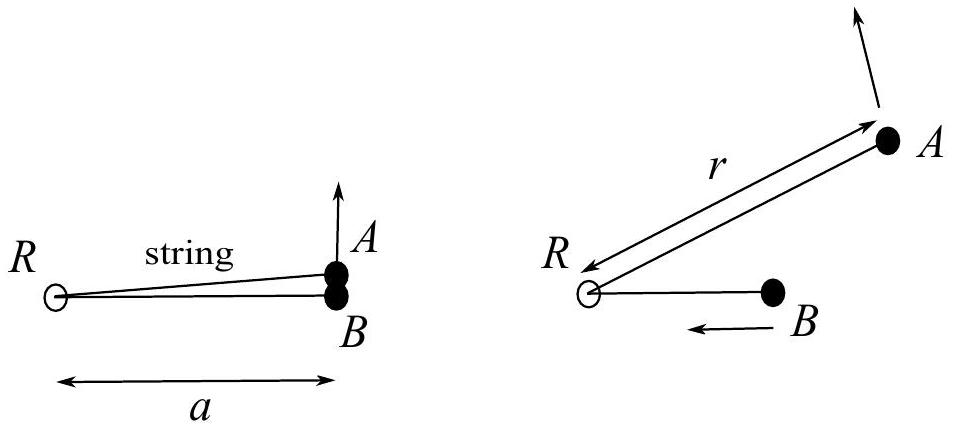
\includegraphics[width=8cm]{sheet 6 diagram}\end{center}
They are connected by a light inextensible string of length $2 a$ which passes through a light ring $R$ fixed in the table at a distance $a$ from the particles. The ring is smooth and can rotate freely. The particle $A$ is given an initial velocity perpendicular to the string in the plane of the table. Show that if $u=1 / r$, where $r$ is the distance of $A$ from $R$, then \[
	\frac{\mathrm{d}^{2} u}{\mathrm{~d} \theta^{2}}+\frac{m_{1}}{m_{1}+m_{2}} u=0,
\] where $\theta$ is the angle $A R B$. Hence find the equation of the path taken by $A$ (up until the moment $B$ reaches $R$). [\emph{Hint}: The tension in the string provides a central force for both particles.]

\end{questions}

\end{document}
